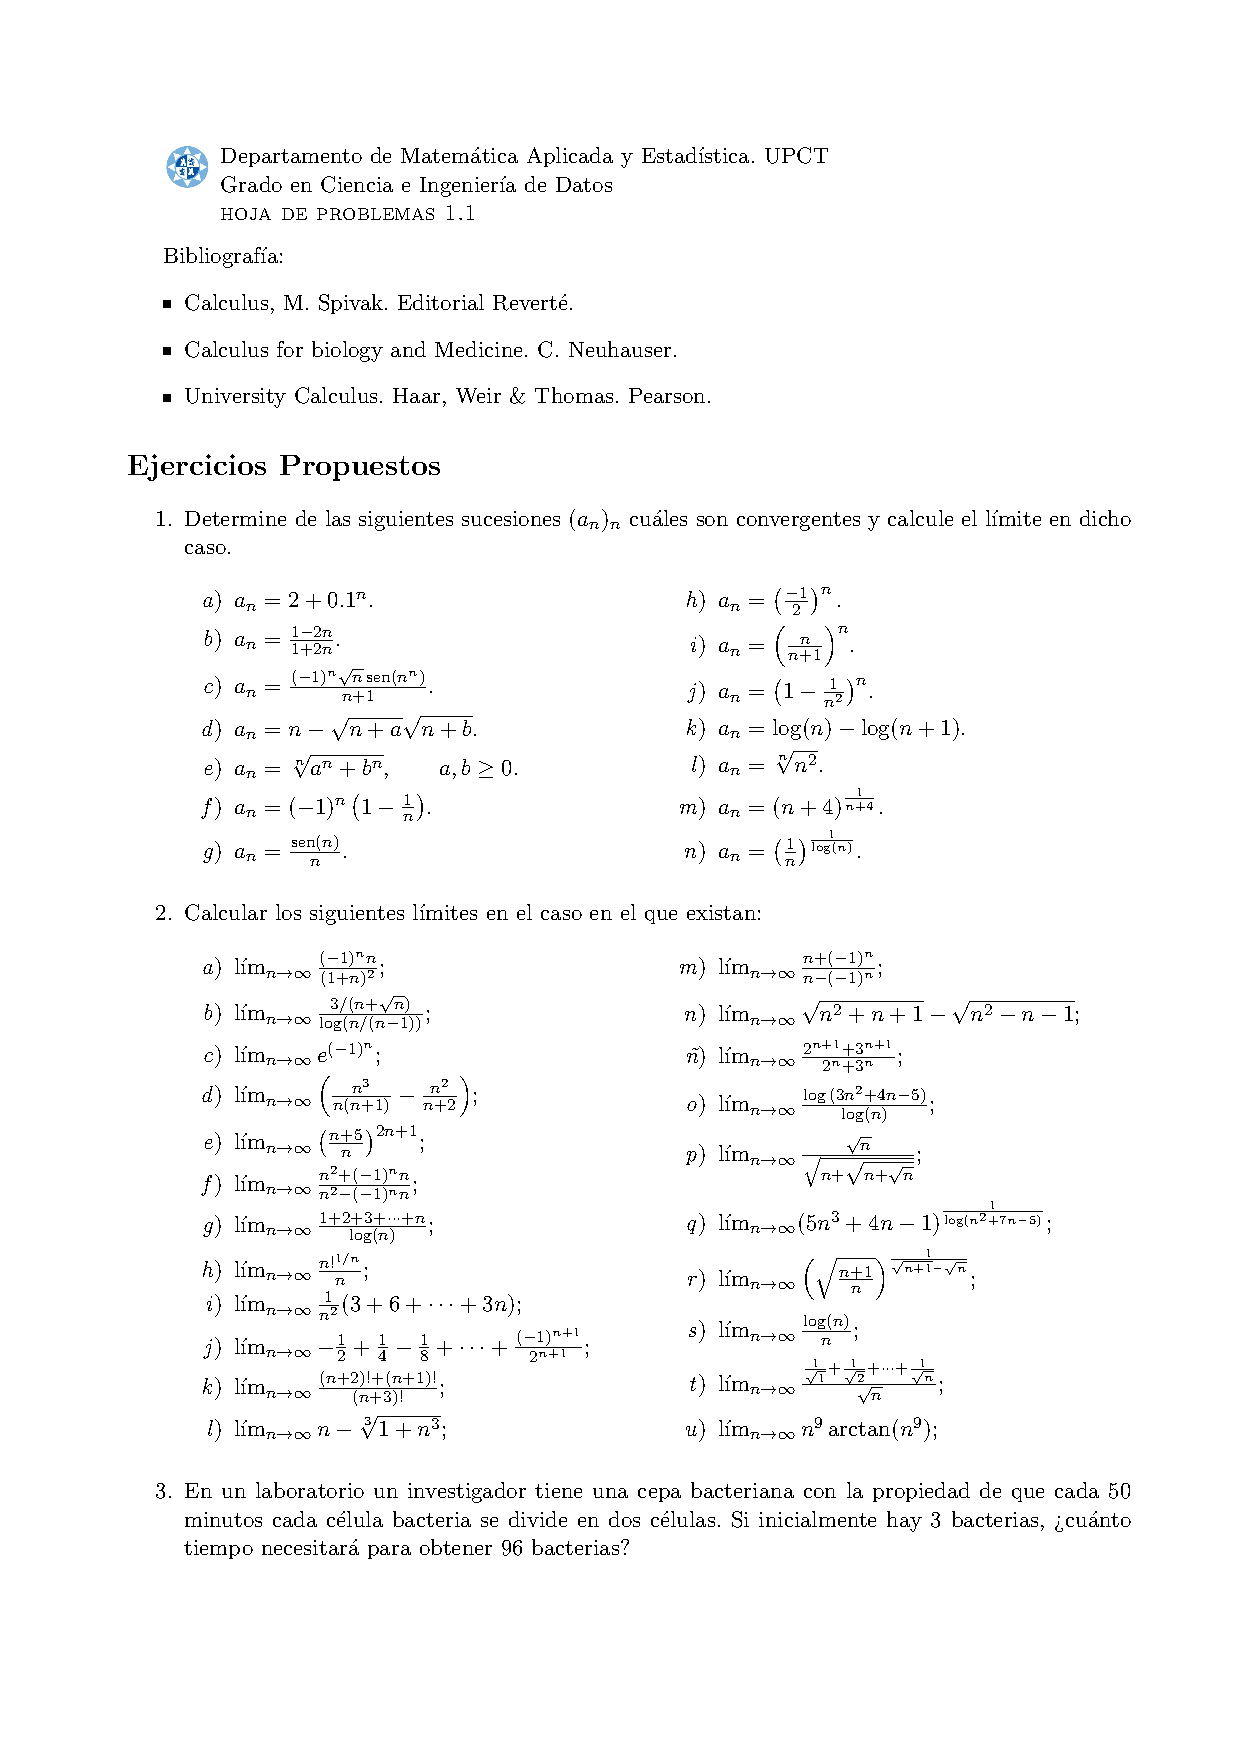
\includepdf[pages=-]{Tema 1/Hoja 1.1/Hoja 1.1.pdf}

\textcolor{red}{1) }\lb{Determine de las siguientes sucesiones $(a_n)_n$ cuáles son convergentes y calcule el límite en dicho caso.}
\begin{enumerate}[label=\color{red}\alph*)]
    \item $\db{a_n=2+0.1^n}$
    \item $\db{a_n=\dfrac{1-2n}{1+2n}}$
    \item $\db{a_n=\dfrac{(-1)^n\sqrt{n}\sin(n^n)}{n+1}}$
    \item $\db{a_n=n-\sqrt{n+a}\sqrt{n+b}}$
    \item $\db{a_n=\sqrt[n]{a^n+b^n},\qquad a,b\ge0}$
    \item $\db{a_n=(-1)^n\left(1-\dfrac{1}{n}\right)}$
    \item $\db{a_n=\dfrac{\sin(n)}{n}}$
    \item $\db{a_n=\left(-\dfrac{1}{2}\right)^n}$
    \item $\db{a_n=\left(\dfrac{n}{n+1}\right)^n}$
    \item $\db{a_n=\left(1-\dfrac{1}{n^2}\right)^n}$
    \item $\db{a_n=\log(n)-\log(n+1)}$
    \item $\db{a_n=\sqrt[n]{n^2}}$
    \item $\db{a_n=(n+4)^{\frac{1}{n+4}}}$
    \item $\db{a_n=\left(\dfrac{1}{n}\right)^{\frac{1}{\log(n)}}}$
\end{enumerate}

\textcolor{red}{2)} \textcolor{lightblue}{Calcular los siguientes límites en el caso en el que existan:}

\begin{enumerate}[label=\color{red}\alph*), leftmargin=*]
	\item $\textcolor{blue}{\lim_{n\to\infty}\dfrac{(-1^nn)}{(1+n)^2}=}$
	\item $\textcolor{blue}{\lim_{n\to\infty}\dfrac{\frac{3}{n+\sqrt{n}}}{\log\left(\frac{n}{n-1}\right)}=}$
	\item $\textcolor{blue}{\lim_{n\to\infty}\mathrm{e}^{(-1)^n}=}$
	\item $\textcolor{blue}{\lim_{n\to\infty}\left(\dfrac{n^3}{n(n+1)}-\dfrac{n^2}{n+2}\right)=}\lim_{n\to\infty}\left(\dfrac{n^3}{n^2+n}-\dfrac{n^2}{n+2}\right)=\lim_{n\to\infty}\dfrac{n^3(n+2)-(n^2(n^2+n))}{(n^2+n)\cdot(n+2)}=$
    
    $\lim_{n\to\infty}\dfrac{\cancel{n^4}+\cancel{2}n^3-\cancel{n^4}-\cancel{n^3}}{n^3+2n^2+n^2+2n}=\lim_{n\to\infty}\dfrac{n^3}{n^3+3n^2+2n}=\lim_{n\to\infty}\dfrac{\frac{n^3}{n^3}}{\frac{n^3}{n^3}+\cancelto{0}{\frac{3n^2}{n^3}}+\cancelto{0}{\frac{2n}{n^3}}}=\bboxed{1}$
	\item $\textcolor{blue}{\lim_{n\to\infty}\left(\dfrac{n+5}{n}\right)^{2n+1}=}$
	\item $\textcolor{blue}{\lim_{n\to\infty}\dfrac{n^2+(-1)^nn}{n^2-(-1)^nn}=}$
	\item $\textcolor{blue}{\lim_{n\to\infty}\dfrac{1+2+3+\cdots+3n}{\log(n)}}$
	\item $\textcolor{blue}{\lim_{n\to\infty}\dfrac{(n!)^{\frac{1}{n}}}{n}=}\left\{n!\equiv\mathrm{e}^{-n}n^n\sqrt{2\pi n}\right\}=\lim_{n\to\infty}\dfrac{\mathrm{e}^{-\frac{n}{n}}n^{\frac{n}{n}}(2\pi n)^{\frac{1}{2n}}}{n}=\lim_{n\to\infty}\mathrm{e}^{-1}{\color{lightblue}\underbracket[1pt]{{\color{black}(2\pi n)^{\frac{1}{2n}}}}_{(\ast)}}=\bboxed{\mathrm{e}^{-1}}$
	
	$\textcolor{lightblue}{(\ast)}=\lim_{n\to\infty}(2\pi n)^{\frac{1}{2n}}=\lim_{n\to\infty}\mathrm{e}^{\frac{1}{2n}\log(2 \pi n)}=\lim_{n\to\infty}\mathrm{e}^{\frac{\log(2\pi(n+1))-\log(2\pi n)}{2(n+1)-2n}}=\lim_{n\to\infty}\mathrm{e}^{\frac{\log(\frac{2\pi n+2\pi n}{2\pi n})}{2}}=1$
	
	\item $\textcolor{blue}{}$
	\item $\textcolor{blue}{}$
	\item $\textcolor{blue}{}$
	\item $\textcolor{blue}{}$
	\item $\textcolor{blue}{}$
	\item $\textcolor{blue}{\lim_{n\to\infty}\sqrt{n^2+n+1}-\sqrt{n^2-n-1}=}\lim_{n\to\infty}\sqrt{n^2+n+1}\left(1-\sqrt{\dfrac{n^2-n-1}{n^2+n+1}}\right)=$
	
	$\lim_{n\to\infty}\sqrt{n^2+n+1}\left(1-\left(1+\underbrace{\dfrac{n^2-n-1}{n^2+n+1}-1}_{a_n}\right)^{\frac{1}{2}}\right)=\lim_{n\to\infty}\sqrt{n^2+n+1}\left(\dfrac{1}{\cancel{2}}\cdot\dfrac{\cancel{2}(n+1)}{n^2+n+1}\right)=\dfrac{n^2-n-1}{n^2+n+1}-1=\dfrac{-2n-2}{n^2+n+1}=\bboxed{1}$
\end{enumerate}

\textcolor{red}{3) }\textcolor{lightblue}{En un laboratorio un investigador tiene una cepa bacteriana con la propiedad de que cada 50 minutos cada célula bacteriana se divide en dos células. Si inicialmente hay 3 bacterias, ¿cuánto tiempo necesitará para obtener 96 bacterias?}

$\begin{array}{l}
	x_{n+1}=2\cdot x_n\\
	x_1=3\\
	x_2=6\\
	
\end{array}$

\textcolor{red}{4)} \textcolor{lightblue}{Un ahorrador dispone de 10000 euros y le ofrecen un interés del 2\% anual. ¿Cuánto dinero tendrá cuando hayan transcurrido 3 años?}

$\begin{array}{l}
	C_0=10000 \qquad 2\%\\
	C_1=10000(1+0.02)\\
	C_2=1.02\cdot C_1=1.02^2 \cdot C_0\\
	C_3=1.02\cdot C_2=1.02^3\cdot C_0
\end{array}$

\textcolor{red}{5) }\textcolor{lightblue}{Resuelve los siguientes apartados:}

\begin{enumerate}[label=\color{red}\alph*), leftmargin=*]
	\item \textcolor{blue}{ Demuestre que si $0<a<2$, entonces $a<\sqrt{2a}<2$.}
	
	$\begin{array}{l}
		a<2\xrightarrow{a>0}a^2<2a\xrightarrow{\sqrt{x}}\sqrt{a^2}<\sqrt{2a}\xrightarrow{a>0}a<\sqrt{2a}\\
		a<2\longleftrightarrow 2a<4\xrightarrow{\text{es creciente}}\sqrt{2a}<2
	\end{array}$
	
	\item \textcolor{blue}{Demuestre que la sucesión \[ \sqrt{2}<\sqrt{2\sqrt{2}},\sqrt{2\sqrt{2}\sqrt{2}},\hdots, \] converge.}
	
	$a_1=\sqrt{2}\qquad a_ 2=\sqrt{2\sqrt{2}}$
	
	\boxed{\begin{array}{l}
		a_{n+1}=\sqrt{2a_n}\\
		a_{n+1}\ge a_n\\
		\sqrt{2a_n}\ge a_n
	\end{array}} Monótona crecietne acotada superiormente
	
	Inducción: $a_n\ge a_{n-1}$ \[ a_{n+1}=\sqrt{2a_n}\ge \sqrt{2a_{n-1}=a_n} \]
	\item \textcolor{blue}{Halle el límite.}
	
	$\begin{array}{ccc}
		\underset{\downarrow}{a_{n+1}} & = & \underset{\downarrow}{\sqrt{2a_n}}\\
		l & & l
	\end{array}$
	
	$\begin{array}{l}
		l(l-2)=0\\
		l^2-2l=0\\
		l^2=2l\\
		a<\sqrt{2a}
	\end{array}$
\end{enumerate}

\textcolor{red}{6) }\textcolor{lightblue}{Sea $(x_n)_n$ una sucesión definida por $x_1=1$ y $x_{n+1}=\sqrt{1+x_n}$ para cada $n\ge1$. Demostrar que la sucesión $(x_n)_n$ es convergente demostrando que es monótona creciente y acotada superiormente. Hallar $\lim_{n\to\infty}x_n$.}

$\begin{array}{l}
	x_1=1\\
	x_{n+1}=\sqrt{1+x_n}
\end{array}$

Monótona creciente (inducción) acotada superiormente

$\begin{array}{l}
	x_1=1\\
	x_2=\sqrt{1+1}=\sqrt{2}>x_1\\
	x_n\ge x_{n-1}\text{ (Hipótesis de inducción)}\\
	x_{n+1}=\sqrt{1+x_n}\ge\sqrt{1+x_{n-1}}=x_n\\
	x_n\ge 0
\end{array}$

\begin{tikzpicture}[baseline=(current bounding box.center)]% function
	\begin{axis}[xlabel=x,ylabel=y, axis lines=center]
		\addplot[domain=-1:1, samples=150, lightblue] {x^2};
	\end{axis}
\end{tikzpicture}

\textcolor{red}{7)} \textcolor{lightblue}{Calcula el límite de las siguientes sucesiones recurrentes, comprobando previamente su existencia.}

\begin{enumerate}[label=\color{red}\alph*), leftmargin=*]
	\item $\textcolor{blue}{x_1=1,x_{n+1}=\sqrt{\dfrac{3x_n+2}{2}}}$
	\item $\textcolor{blue}{x_1=1,x_{n+1}=\dfrac{4}{4-x_n}}$
	
	$\begin{array}{l}
		x_1=1\\
		x_{n+1}=\dfrac{4}{4-x_n}
	\end{array}$
	
	Monótona creciente (inducción)
	
	$x_2=\dfrac{4}{4-1}=\dfrac{4}{3}>x_1=1$
	
	$\begin{array}{l}
		x_n> x_{n-1}\\
		-x_n\le -x_{n-1}\\
		4-x_n\le 4-x_{n-1}\\
		\dfrac{1}{4-x_n}\ge \dfrac{1}{4-x_{n-1}}
	\end{array}$
	
	$x_{n+1}=\dfrac{4}{4-x_n}\ge\dfrac{4}{4-x_{n-1}}=x_n$
\end{enumerate}